\section{Foundational Concepts}
\label{sec:concepts}

\rx is an adaptive, artificial intelligence based controller and
provides general framework for building reasoning systems for
real-world autonomous vehicles. At MBARI \rx is used for AUV control;
another instantiation of the system is being used for control of a
terrestrial personal robot \cite{pr2, Meeussen:2010dn}. The
development of \rx has been targeted at surveying a number of
oceanographic features which are dynamic and unpredictable
spatio-temporally. Typically this requires our AUVs to balance the
goals of coverage spatially while opportunistically following features
of scientific interest and to do so while being operationally aware of
its own limitations in terms of resources (typically the battery state
of charge) and overall proximity to other observational assets for
obtaining scientific ground-truth. We are therefore interested in
representational frameworks that allow robots to pursue long-term
objectives while choosing short-term gain and can gracefully deal with
exogenous or endogenous change.

To enable this responsiveness to external observations, the agent has
to be able to synthesize plans insitu and to re-plan. We use a
temporal constraint-based planner \eu with a demonstrated legacy of
having flown on NASA space missions \cite{jonsson00,bresina05,
  barreiro09}. Our autonomy architecture brings three key innovations
for AUV adaptation: the use of flexible plan representations,
compositional control with the use of partitioned networks and
off-line learning to inform insitu environmental state estimation. In
this section we detail some of the key concepts relevant to flexible
plan representation. Section \ref{sec:arch} has details the
\rx partitioned architecture and estimation driven vehicle
adaptation.

\subsection{The basics}
\label{sec:basics}

\eu uses a \emph{domain model} written in a declarative language
(NDDL: New Domain Description Language), together with initial
conditions and goals also specified in NDDL, to construct a set of
temporal relations that must be true at the start time. These models
include assertions about the physics of the vehicle, i.e how it
responds to external stimulus and internally driven goals. By
propagating these relations forward using Simple Temporal Networks
\cite{dechter91} and applying goal constraints, \eu can select a set
of conditions that should be true in the future, where some of these
conditions will correspond to actions the agent must take. The planner
can backtrack and try another path during search if a goal cannot be
reached while being capable of discarding unachievable goals.

Traditionally robot execution has relied on dispatching commands at
precise times. Such linear sequences of precisely timed commands give
no ability to adjust execution on the basis of sensory
information. Although some commands can issue tests on sensor
readings, these tests have the objective of verifying whether expected
execution conditions are occuring. If not, the state of the system is
declared off-nominal and execution of the sequence of commands is
interrupted. More recently, executives have been proposed and
implemented that significantly broaden the way robots can be commanded
\cite{mus98,alami:1998p820}. For example, the Remote Agent executive
interpreted a \textit{temporally flexible plan} which represents each
start time as a variable and contains an explicit network of bounded
delay constraints between such variables.

\begin{figure}[!t]
\centering
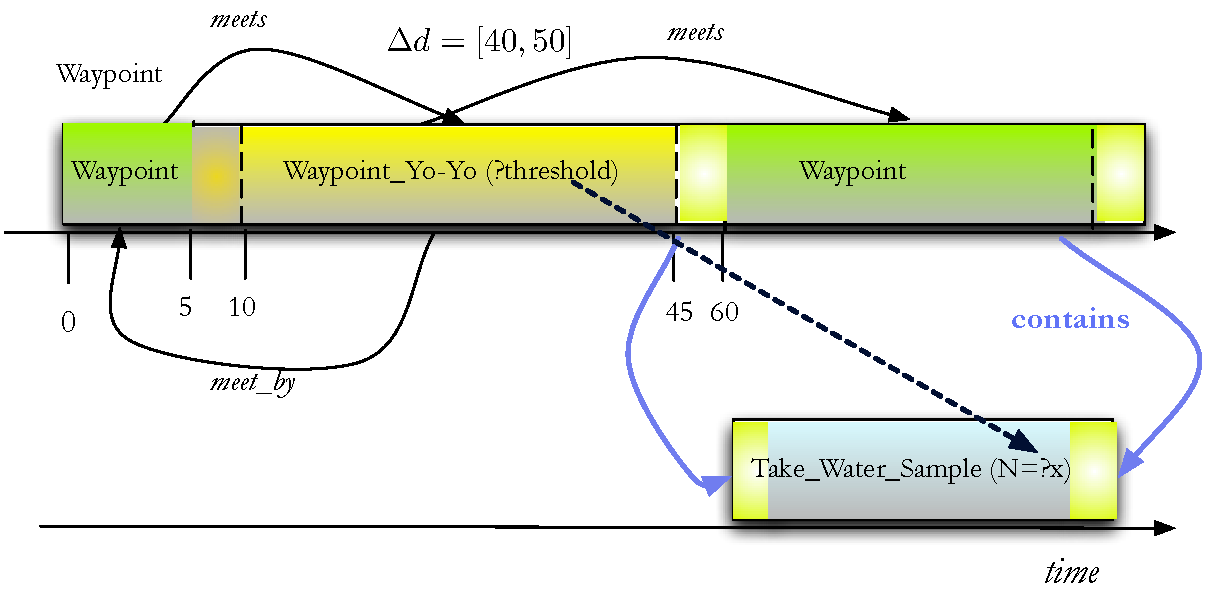
\includegraphics[scale=0.35]{figs/flexible-timelines.pdf}
\caption{\small Tokens with flexible temporal intervals and parametric
  constraints between tokens. This example shows the triggering of a
  water sampler based on a feature threshold while the vehicle
  Yo-Yo's. The \texttt{Waypoint\_Yo-Yo} token has a flexible duration,
  start \& end times.}
\label{fig:flex-timelines}
\vskip+0.1cm
\end{figure}

Unlike a traditional fixed time-tagged command sequences, such
flexible plans leave room for adaptation at execution time. When the
executive considers when to start a task, it propagates information
through the constraint network, computes a time bound for the
variable, selects an actual execution time within the bound, and
starts the task at that time. Temporally flexible plans therefore,
express a \textit{range of possible outcomes} of the robots
interaction with the environment within which the executive can elect
at run time the most appropriate one for the actual execution
conditions. The fact that constraints are explicitly represented
ensures that through constraint propagation the executive will respect
global limits expressed in the plan (e.g., don't start a task until a
certain condition has been satisfied but still satisfying some global
deadline). Such flexibility is critical when dealing with dynamic
ocean conditions where precise timing of a robotic action might be
indeterminate. Further, the advantage of flexibility can be contrasted
with the consequences of the intrinsic inflexibiliy of traditional
command sequences. Because they are inflexible, sequences must
necessarily be designed considering worst case scenarios.

\eu uses a \emph{state variable} representation to describe the
evolution of state over time. The instantiated history of such state
variable evolution over a temporal horizon we call \emph{timelines}
and which represent a single thread in the execution of a concurrent
system. At any given time each thread can execute a single procedure.
Thus each timeline consists of a sequence of procedures which
encapsulate and describe state evolution; we call these instantiated
atomic entities \emph{tokens}.  A token therefore describes a
procedure invocation, the state variables on which it can occur, the
parameter values of the procedure, and the time values defining the
interval. We allow encapsulation of uncertainty within these tokens
with a range of start and end times and parameters, all of which are
encoded as variables. A constraint solver in turn manipulates these
variables defined in a \eu domain model. For example, consider
a scientific need to take a water samples 100 meters from a hotspot
while an AUV is performing a Yo-Yo in the water-column. Two samples
are needed if the feature's signal is above a threshold; one
otherwise. The token that is capturing the sensory threshold has a
parametric constraints to the token which fires the requisite water
sampler. In addition, the start time of the water sampling procedure
is highly dependant on the variability of sub-sea currents and actual
speed of the vehicle. Therefore a number of values are possible for
the start times and duration of the sampling all of which are valid
combinations for desired outcomes.

% \begin{figure}
% \centering
% 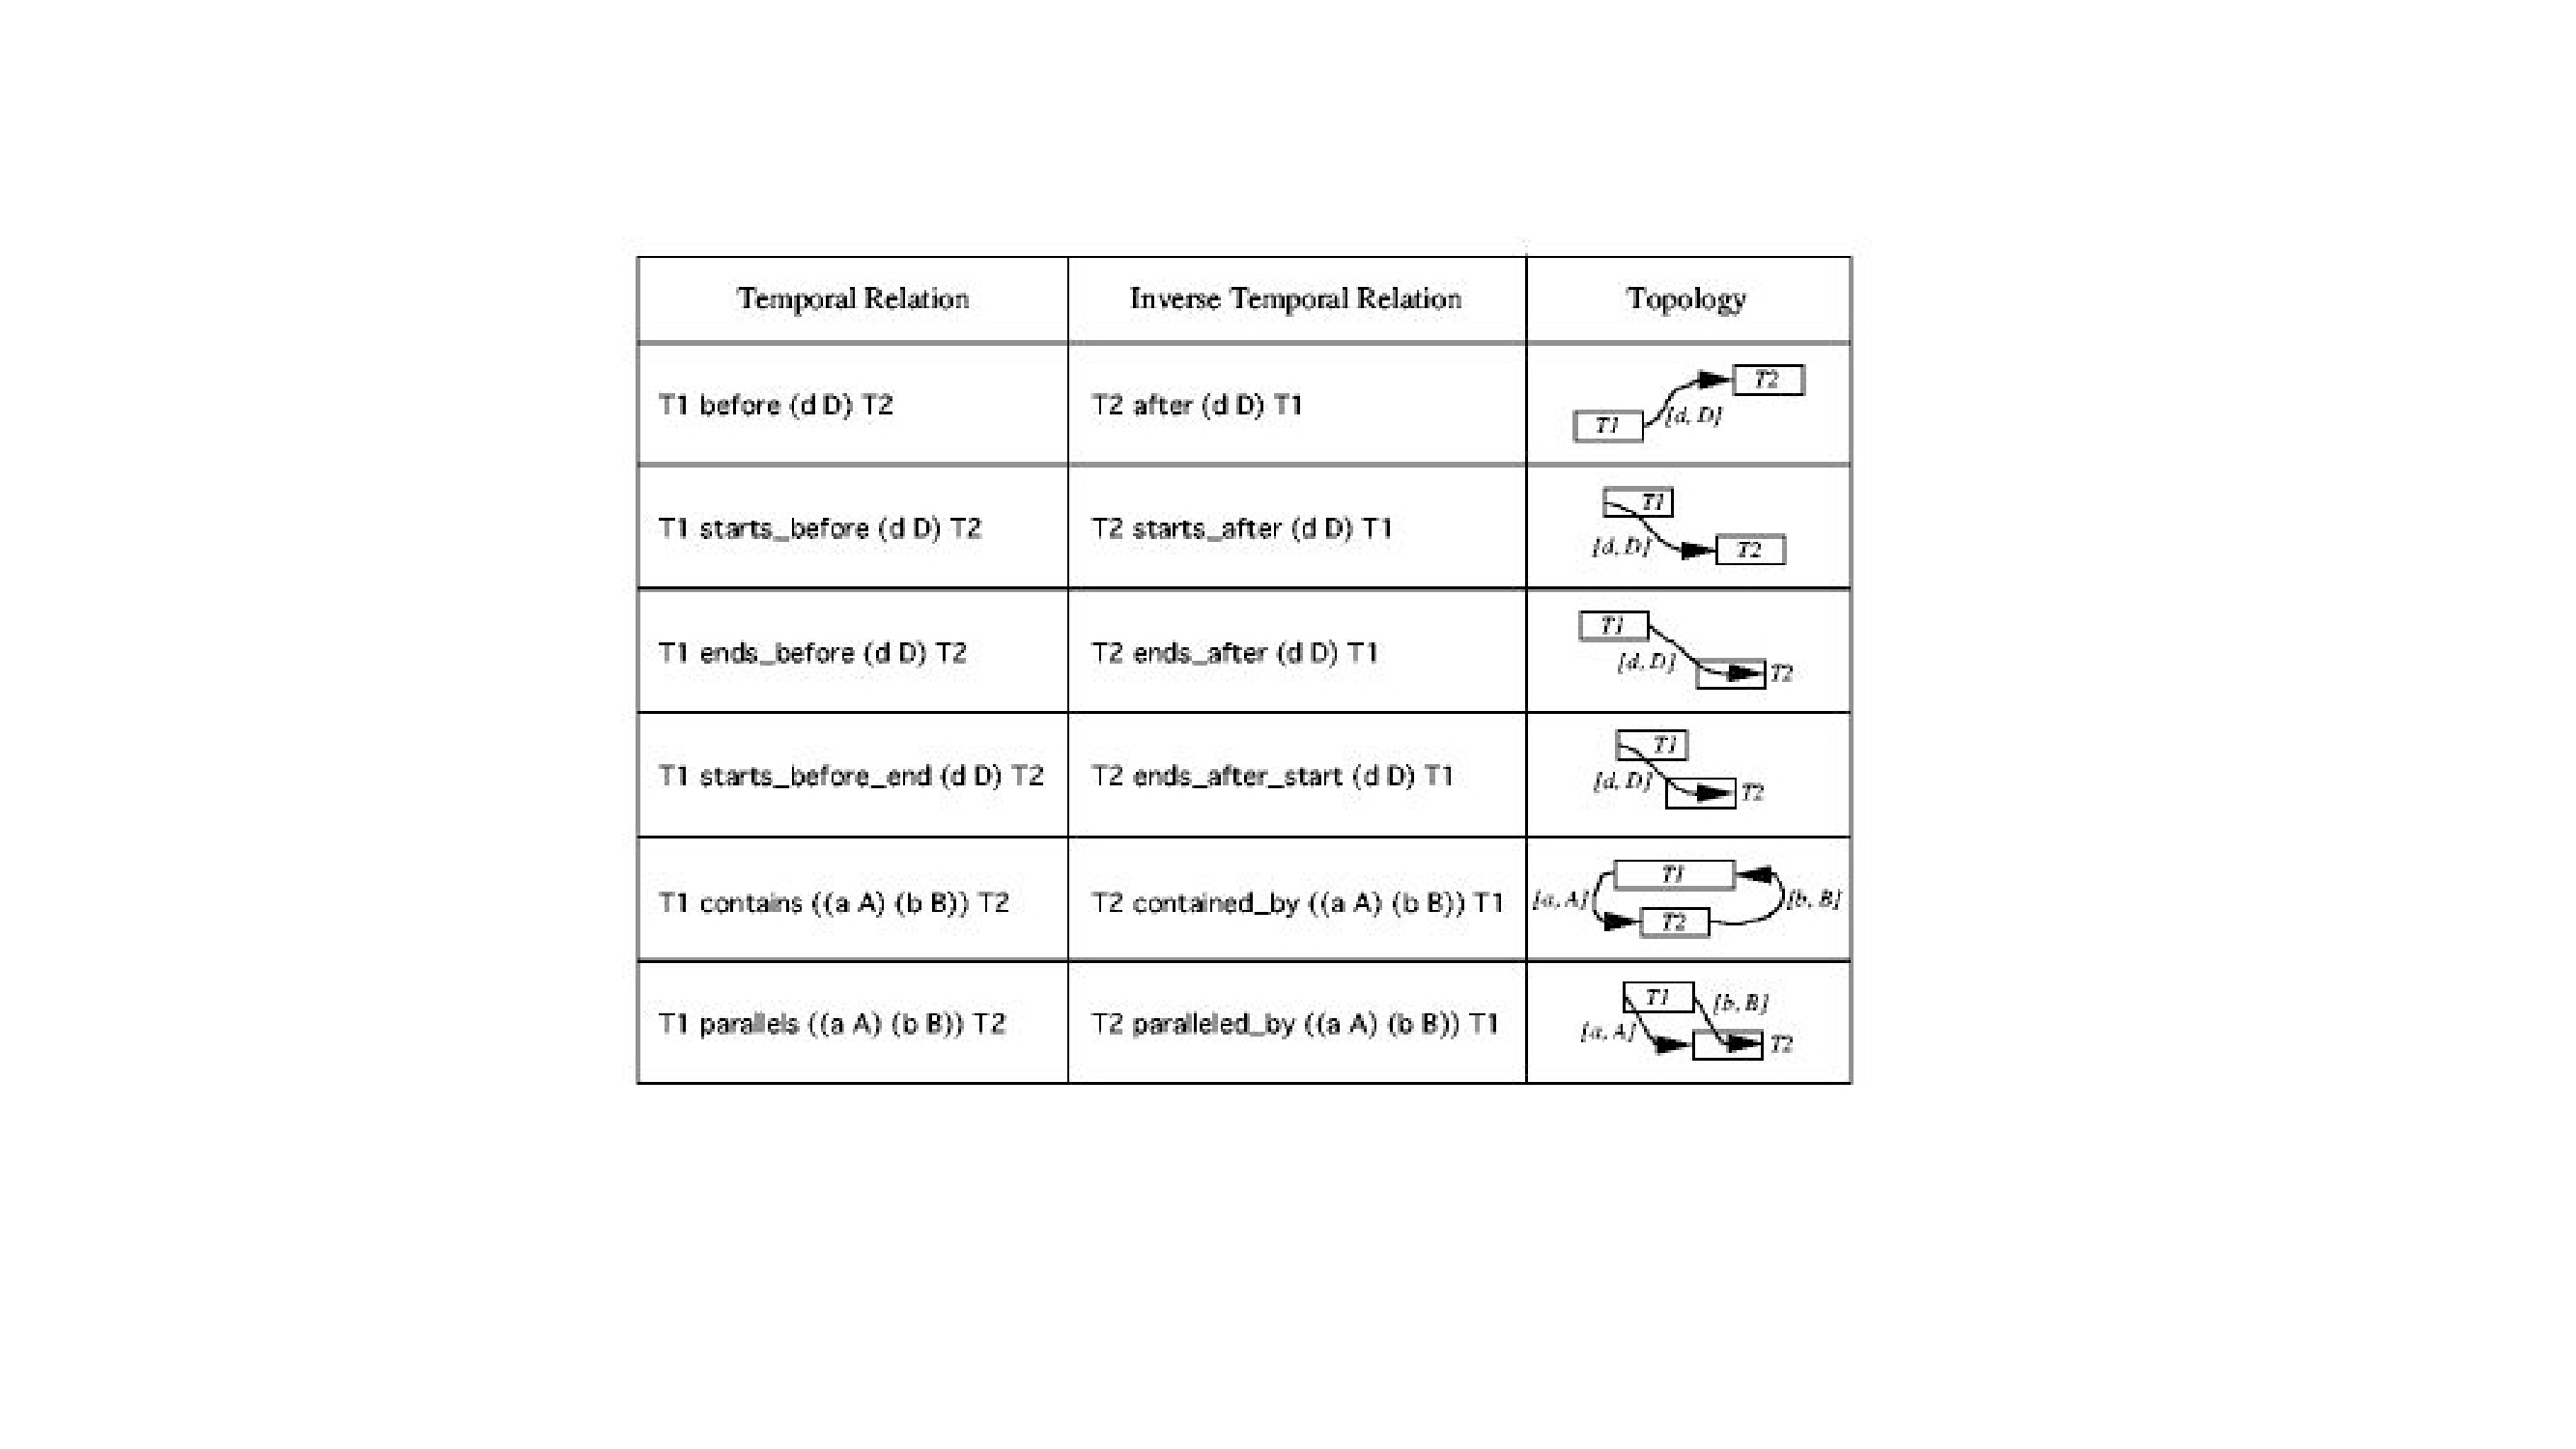
\includegraphics[scale=0.3]{figs/Allen-algebra.pdf}
% \caption{\small Temporal relations defined within the planner are
%   based on \texttt{Allen Algebra} relations shown above.}
% \label{fig:allen-algebra}
% \vskip-0.3cm
% \end{figure}

\section{Fundamentals of  Automated Planning}
\label{sec:europa}

{\footnotesize
  \begin{quote}
[Planning] \emph{is an abstract, explicit deliberation process that chooses and
organizes actions by anticipating their expected outcomes. This
deliberation aims at achieving as best as possible some prestated
objectives. Automated planning is an area of Artificial Intelligence
(AI) that studies this deliberation process computationally.} -- from
\textbf{Automated Planning Theory and Practice} by Ghallab, Nau and
Traverso \cite{ghallab04} 
\end{quote}
}

% Planning, for our purposes, can be thought of as determining all the
% small tasks that must be carried out in order to accomplish a goal.
To articulate the fundamentals of automated planning briefly and use
that to motivate the mechanisms we use in our specific form of the
technique we start with a simple example.

\begin{quotation}

  In the near future, a personal robot sets out to buy a gallon of milk
  This involves a number of tasks: obtain keys, obtain wallet,
  start car, drive to store, find and obtain milk, purchase milk, etc.
  The embedded planner has to have a ``model'' of the world in which it
  lives and has to use the task primitives in this model to structure
  the actions so it achieves its goal. Constraints control when certain
  tasks can or cannot occur. For example the robot must obtain the keys
  and wallet \emph{before} driving to the store and pick up the milk
  \emph{before} purchasing it.

\end{quotation}

For such a robot the milk buying plan at the store might look like
\comment{Figure needed}.

At the core of the \rx framework, is the deliberation engine, \eu,
which has a rich legacy from NASA missions. \eu is a versatile
Constraint-based temporal planner which continues to be deployed on a
diverse set of applications. We motivate this section with some
problem domains this planner can handle and then delve in substantial
detail.

\paragraph \textit{Constraint Satisfaction}: A canonical problem in
dealing with constraints is the $N$-Queens problem in which chess queens
must be placed on an  $N$x$N$ chessboard so no queens attack the other. Fig.
\ref{fig:nqueens-1} shows an example of a random positioning of queens
on a  $N$x$N$ chessboard. Queens in violation of the non-attack constraint
are highlighted in red.

\begin{figure} \centering
  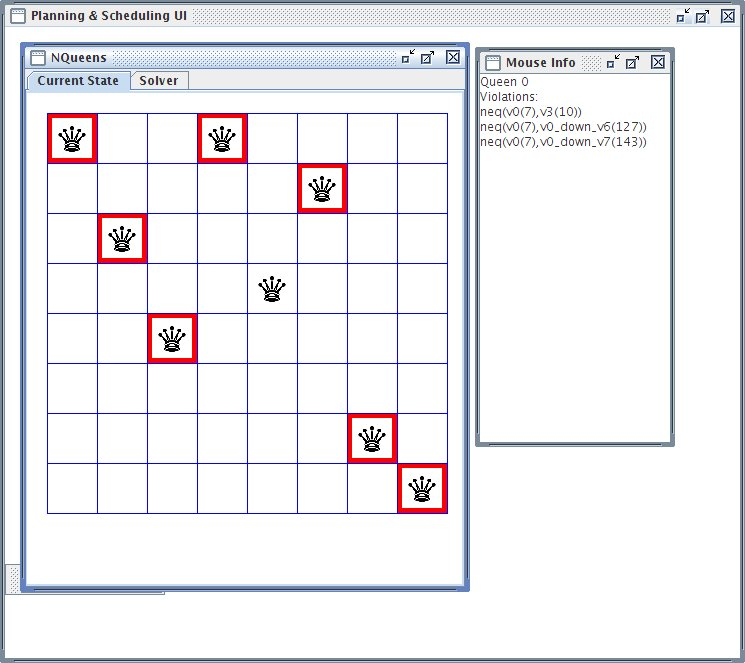
\includegraphics[scale=0.35]{figs/Example-NQueens0.jpg}
  \caption{\small N-Queens problem. Queens in violation of the
    non-attack constraint are highlighted in red.}
\label{fig:nqueens-1}
\vskip+0.1cm
\end{figure}


If we define $N$x$N$ variables Q$_{rc}$, $r \in [1,N]$, $c \in [1,N]$,
Q$_{rc} = 1$ if cell $r,c$ in the chessboard is occupied by a Queen, $0$
otherwise. Then the following constraints need to be satisfied:

\begin{equation}
 Sum(Q_{rc})= \left\{
\begin{array}{l l}
  1 & \forall r \quad \mbox{(only one Queen per row)}\\
  1 & \forall c \quad \mbox{(only one Queen per column)}\\ 
\end{array} \right.
Sum(Q_{r+i,c+i}) = 1\\
Sum(Q_{r-1,c+i}) = 1 \quad \mbox{(only one Queen on each diagonal)}\\
\end {equation} 

\comment{fix newline and numbering problem above}

The problem can be solved by finding assignments for all variables
Q$_{rc}$ that satisfy the above constraints. Fig. \ref{fig:nqueens-2} is
a solution found by \eu using that formulation and a specialized search
procedure.

\begin{figure}
\centering
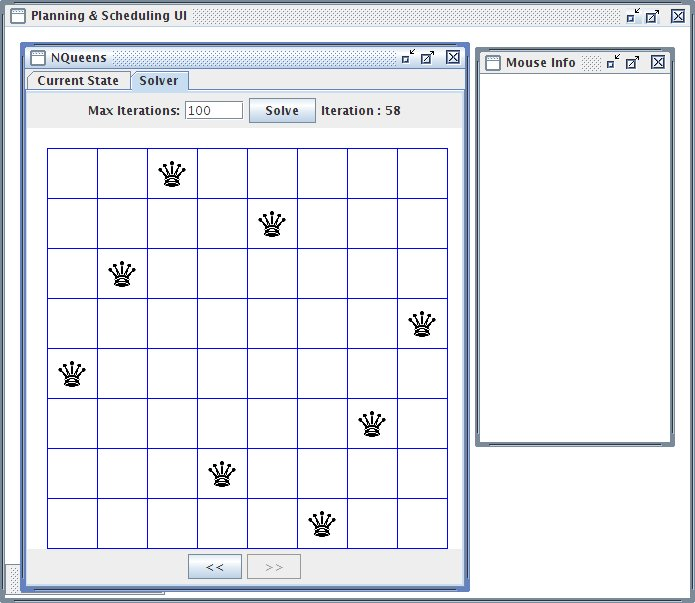
\includegraphics[scale=0.35]{figs/Example-NQueens1.jpg}
\caption{\small N-Queens solution generated by \eu}
\label{fig:nqueens-2}
\vskip+0.1cm
\end{figure}


\paragraph \textit{Scheduling}: In the Resource Constrained Project
Scheduling Problem (RCPSP) \cite{Bruckera99}, a project consisting of
a set of activities must be scheduled in a way that satisfies minimum
and/or maximum temporal separation constraints. The activity schedule
must also respect fixed limits on the availability of resources
required to perform each activity. In addition to satisfying temporal
and resource constraints, it is common for the user to want to
minimize makespan so that the entire project is finished as early as
possible. Fig. \ref{fig:rcpsp-1} shows an example of a a solution
provided by \eu for an RCPSP instance with 10 activities, 5 resources
and 30 temporal constraints.

\begin{figure}
\centering
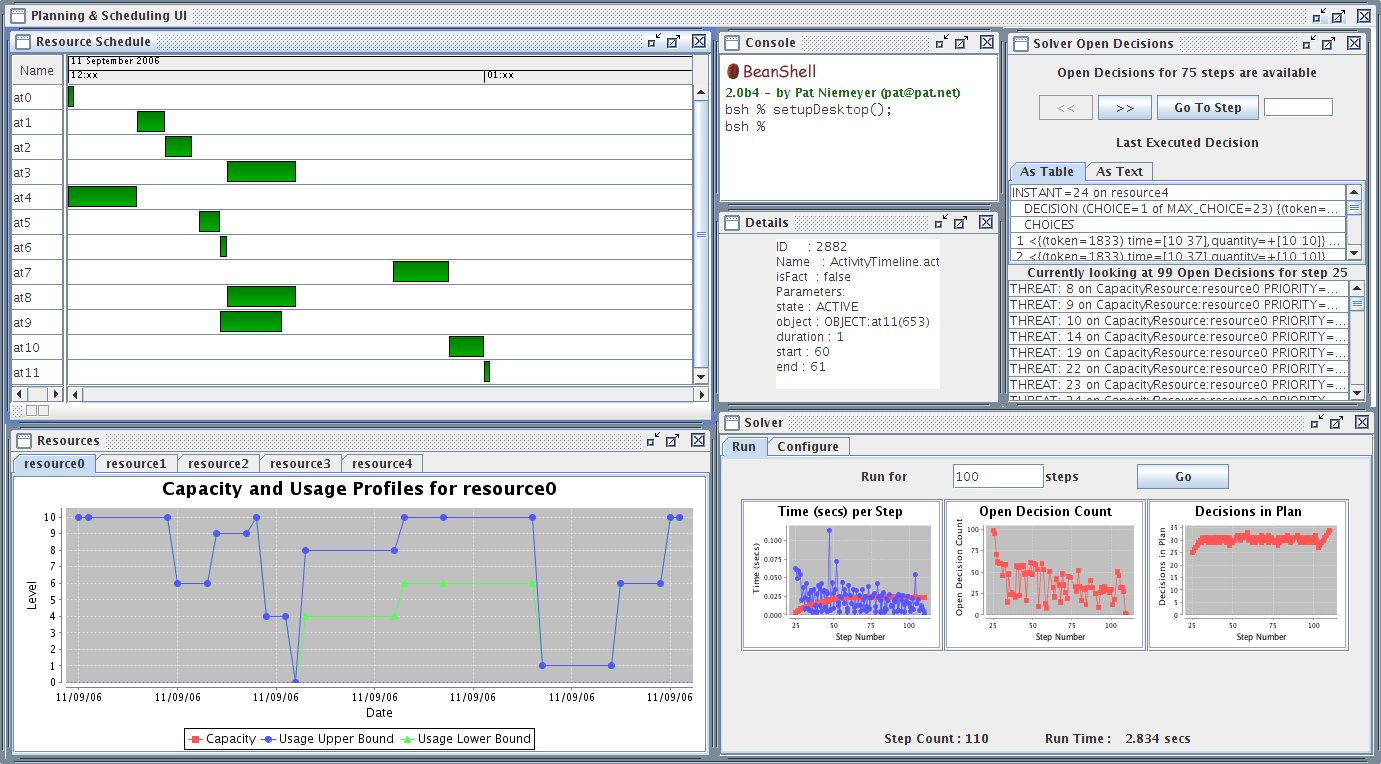
\includegraphics[scale=0.35]{figs/Example-UBO0.jpg}
\caption{\small A \eu solution to an RCPSP \cite{Bruckera99} problem.}
\label{fig:rcpsp-1}
\vskip+0.1cm
\end{figure}


\paragraph \textit{Planning}: In the Shopping Agent Problem
\cite{russelnorvig} an agent needs to purchase a set of products (milk,
drill, etc) that are available at specific locations (supermarket,
hardware store, etc), the agent is subject to temporal (must complete
tasks by specific deadlines) and resource (fuel, carrying capacity, etc)
constraints. The agent needs to figure out what actions need to be
performed to find and acquire the required items, as well as when to
perform each of those actions. Fig. \ref{fig:shopping-1} shows a
solution produced by \eu for such a problem instance.

\begin{figure}
\centering
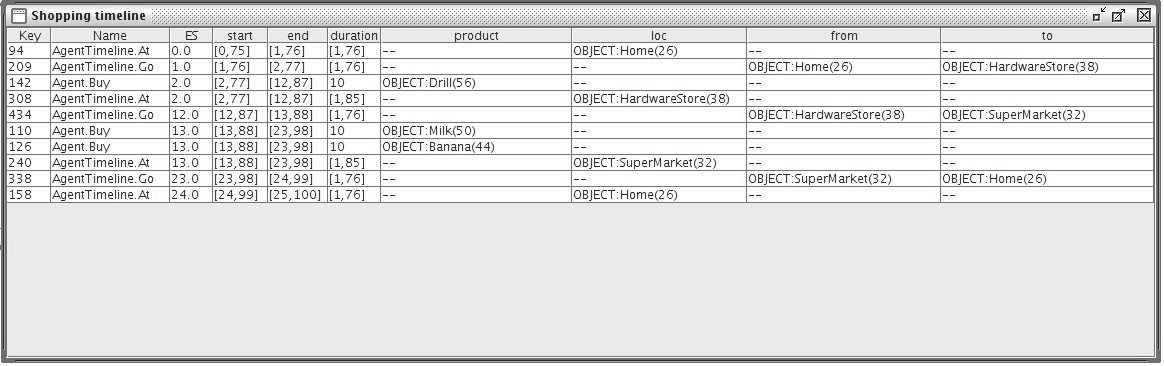
\includegraphics[scale=0.35]{figs/Example-Shopping0.jpg}
\caption{\small A \eu solution to a shopping agent problem domain where
  the agent needs to buy Bananas, Milk and a Drill.}
\label{fig:shopping-1}
\vskip+0.1cm
\end{figure}

As the examples above show, a Planning problem (actions to achieve a
goal) may embed a Scheduling problem (what resources are necessary to
achieve stated goals) and both Planning and Scheduling may embed a
Constraint Satisfaction problem. 
The relationships between Planning, Scheduling and Constraint
Satisfaction have been examined \cite{smith00} and have lead to use of
constraint reasoning in \eu as its innermost building block. 

\subsection{Constraint Programming}
\label{sec:europa:cp}

Constraint Satisfaction Programming (also known as Constraint
Programming (\textsf{CP})) is a discipline that provides a generic framework
for representing, solving and making logical inference on
constraints. A complete treatment of this discipline is given in
\cite{marriott98,apt03} and very concise introductions are provided in
\cite{bartak99,lustig01}.

A constraint programming problem consists of a set of variables $V=
{x_1,..,x_N}$, where each variable takes values from a domain
$d_1,..,d_N$; in this chapter we will deal only with discrete and
finite domains. Given a defined conjunctive set of constraints on the
variables: $C=\{c_1(x_1,..,x_N), ..., c_K(x_1,..,x_N)\}$, the
objective is to find one or more value assignments to $V$ where all
constraints are satisfied. To solve a problem, \textsf{CP} techniques use
logical inference to perform Constraint Propagation, which consists of
two operations:

\begin{enumerate}

\item \textbf{Bounds propagation}: To infer upper and lower variable
  bounds. For example, from the constraints $x_1 + x_2 \leq 2$ \&
  $x_i \geq 0$, we can infer $[0,2]$ bounds for $x_1$ and $x_2$

\item \textbf{Domain reduction}: To infer a valid set of values for a variable.
  For example, for  constraints allDifferent($x_1,x_2,x_3$), $x_i \geq
  0$ \& $x_i \leq 4$, if $x_1 = 1$ and $x_2 = 3$ we can infer that the
  valid domain for $x_3$ is reduced  to $\{2,4\}$

\end{enumerate}

A set of constraints and variables that describe a problem domain are
typically represented as a Constraint Network, where the variables are
nodes and constraints are arcs between the variables. Having this
network representation in mind, a pair of variables $x,y$ is said to
be arc consistent if for every value in $x$'s domain, there is a value
in $y$'s domain that is consistent with all the constraints that
connect $x$ and $y$.  A naive approach to ensuring arc consistency
consists of cycling through all the variable pairs and performing
constraint propagation until there are no variable domain changes. The
AC-3 algorithm \cite{mackworth77}, a popular implementation, improves
over the naive approach by ignoring constraints whose variables were
not affected since the last iteration. \comment{A figure of a
  constraint network preferably of the shopping example would be
  useful here. JB to generate a napkin fig}

Arc Consistency and other, more stringent consistency definitions can
be used to efficiently prove that a \textsf{CP} problem is
unsatisfiable. However, they generally cannot prove that a \textsf{CP}
problem is satisfiable and provide specific variable assignments that
constitute solutions. For that, search algorithms like global
backtracking \comment{citation needed} or local search are used; these
use consistency as an efficient way to prune the search space
\cite{cp06}. In theory, solving a \textsf{CP} problem is NP-Hard
\cite{ghallab04}, but often very efficient in practice using a number
of consistency and search algorithms that are well understood.

\textsf{CP} is usually implemented as part of a programming language
and constraints are usually represented as objects \cite{puget95}. Any
constraint that the user is able to reason about can be introduced
into the system and, as long as the constraint propagation protocols
specified by the host \textsf{CP} system are enforced, it will be
indistinguishable from any other "primitive'' \textsf{CP} constraint,
such as $\leq$ or $\geq$.

\subsection{Constraint-Based Planning}
\label{sec:europa:cp}

The most common planning formulations use a propositional
representation, where the state of the world is represented by a set
of propositions (statements that can be true or false), and operators
change the truth values of these propositions \cite{gen87}. Although
these formulations are powerful and have allowed researchers to
develop numerous contributions in automated planning, there are many
classes of problem domains that are difficult to represent using this
formalism. In particular, it is hard to represent time, resources,

% mutual exclusion and concurrency using propositions
% \cite{ghallab04}. While CSP representations have traditionally had an
% edge in formulating and representing planning problems,
% % It is straightforward to represent and reason about all of
% % those elements using a CSP representation, as a result there has been
% % some work on doing automated planning while taking advantage of CSP
% % (TODO: ref). Traditionally, the entire planning problem is translated
% % into a CSP and then solved using traditional CSP methods, this
% leading to a formulation where action choices and relationships are
% represented as variables and/or constraints, there are at least two
% major drawbacks:

mutual exclusion and concurrency using propositions
\comment{ghallab04}.  Constraint Programming is a framework that lends
itself very well to represent and reason about all of those elements
\comment{Ixtet citation?}, consequently, there has been a good amount
of work building automated planners that take advantage of CP
techniques.  The most common approach in constraint-based planning has
been to encode the entire planning problem as a CP problem, where
action choices and relationships are represented as variables and/or
constraints \comment {citations 158,519,539,556 from malik's book}.
The advantage of using a pure CP formulation is that standard CP
solvers can be then used to solve the planning problem, however, this
approach also has a couple of significant drawbacks:

\begin{enumerate} 

\item Given that action choices and relationships (rules) are expressed
  through variables, the domain descriptions that result from this
  approach are not intuitive and therefore difficult to understand and
  debug

\item If the structure of a planning model (actions, conditions,
  effects, dependencies at the action level) is not explicitly
  maintained by the CSP planner, the search algorithms are deprived of
  critical information to make better decisions. If that structure is
  maintained (for instance, by internally marking variables that
  represent action choice and relationships between actions), it is
  still hard to write search algorithms as any planning-specific
  insight has to be translated into the CSP representation of
  variables and constraints \comment{For example?}

\end{enumerate}

These drawbacks have been addressed by a small number of planning frameworks like Descartes \comment{citation 289,290 from malik's book}, IxTet \comment{citation  223 from Malik's book}, and CAIP (Constraint-Based Interval and Attribute Planning)\cite{mus94,frank2003}.
These frameworks take advantage of a CSP representation to deal with time and resources, at the same time maintaining an explicit representation of the elements relevant to planning (action choices, causal relationships, etc). This combination results in a planning approach that can deal with the type of constraints found in real-life problems, while allowing for intuitive problem descriptions and a natural way to express search algorithms and heuristics. \eu is an implementation of the CAIP framework. In CAIP, planning problems are specified in terms of:

\begin{enumerate}
	\item \textbf{Intervals}: entities that have a temporal scope (that is, a beginning and an  end in time) and a set of attributes. Intervals are used to represent actions and states in the planning domain. 
	\item \textbf{Variables and Constraints}: Variables represent Interval attributes and Constraints enable a direct representation of temporal, resource and any other the restrictions that a valid plan must comply with.
	\item \textbf{Domain Configuration Rules}: this is an explicit representation of the conceptual relationships between actions and states in the problem domain, for instance, for a Shopping Agent to be able to purchase a product, it must be at a location where the product is available.
\end{enumerate}

To generate plans, the CAIP framework uses a plan-space search approach \comment{cite malik's chapter 5}, where a partial plan is evolved until all open goals are achieved, and all inconsistencies are removed, the specific search algorithm used by \eu will be covered in detail below.

